% AgriConnect Architecture Diagram - LaTeX/TikZ Version
% Compile with: pdflatex architecture-diagram.tex
% Requires: tikz, positioning, shapes, arrows

\documentclass[landscape,a4paper,10pt]{article}
\usepackage[margin=1cm]{geometry}
\usepackage{tikz}
\usepackage{xcolor}
\usepackage{fontspec} % For custom fonts (requires XeLaTeX or LuaLaTeX)
\usepackage{float}

\usetikzlibrary{positioning,shapes,arrows,calc,shadows,backgrounds,fit}

% Define colors
\definecolor{hardwaregreen}{RGB}{76,175,80}
\definecolor{gatewayorange}{RGB}{255,152,0}
\definecolor{cloudblue}{RGB}{33,150,243}
\definecolor{aipurple}{RGB}{156,39,176}
\definecolor{dashboardpink}{RGB}{233,30,99}
\definecolor{userpurple}{RGB}{102,126,234}

% Define box styles
\tikzstyle{layer} = [rectangle, rounded corners, minimum width=12cm, minimum height=2cm,
                     text centered, draw=black, line width=0.5mm, fill opacity=0.1]
\tikzstyle{component} = [rectangle, rounded corners, minimum width=3.5cm, minimum height=1.5cm,
                        text width=3.2cm, text centered, draw=black, line width=0.3mm,
                        fill=white, drop shadow]
\tikzstyle{arrow} = [thick,->,>=stealth,line width=1mm]
\tikzstyle{title} = [rectangle, rounded corners, minimum width=3cm, minimum height=0.6cm,
                    text centered, text=white, font=\bfseries]

\begin{document}

\begin{figure}[H]
\centering
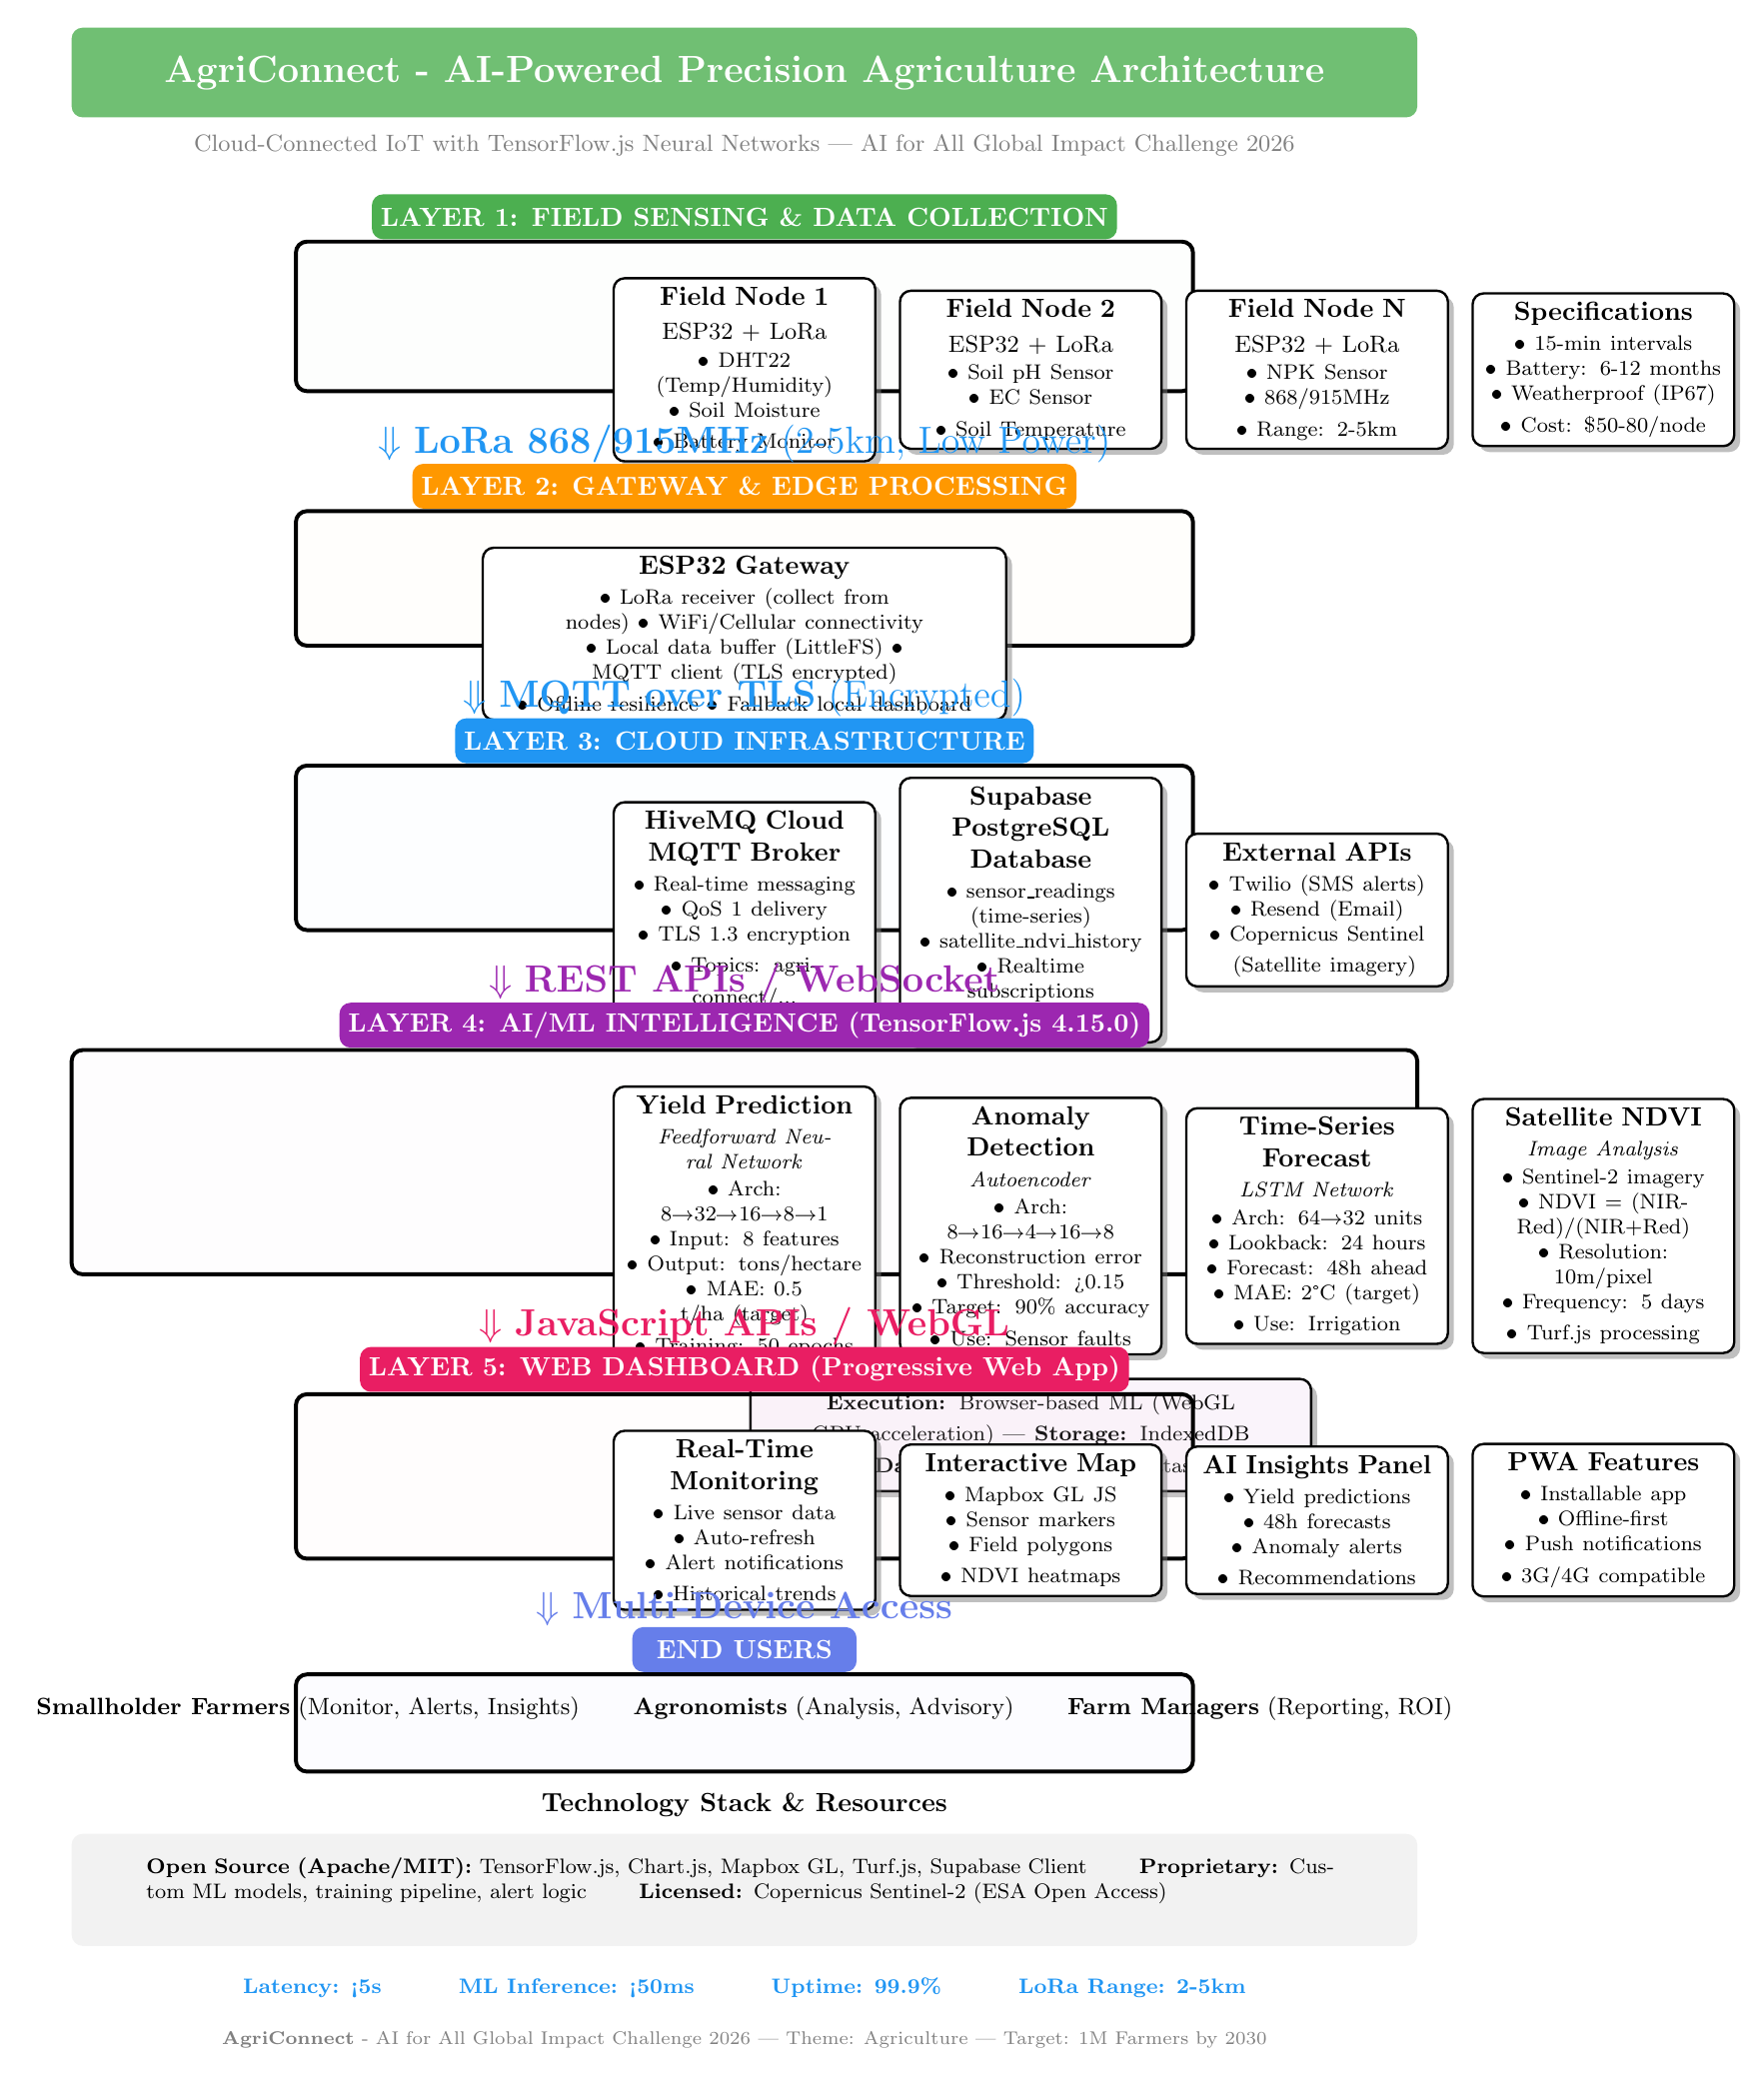
\begin{tikzpicture}[node distance=1.5cm, scale=0.95, transform shape]

% ============= HEADER =============
\node[rectangle, rounded corners, fill=hardwaregreen!80, text=white,
      minimum width=18cm, minimum height=1.2cm, font=\Large\bfseries] (header)
      {AgriConnect - AI-Powered Precision Agriculture Architecture};
\node[below=0.1cm of header, font=\small, text=gray] (subtitle)
      {Cloud-Connected IoT with TensorFlow.js Neural Networks | AI for All Global Impact Challenge 2026};

% ============= LAYER 1: FIELD SENSING =============
\node[layer, fill=hardwaregreen!10, below=1cm of subtitle] (layer1) {};
\node[title, fill=hardwaregreen, above=0cm of layer1.north] (title1) {LAYER 1: FIELD SENSING \& DATA COLLECTION};

% Field components
\node[component, below=0.5cm of title1] (node1) {
    \textbf{Field Node 1}\\[2pt]
    \small ESP32 + LoRa\\[1pt]
    \footnotesize • DHT22 (Temp/Humidity)\\
    \footnotesize • Soil Moisture\\
    \footnotesize • Battery Monitor
};

\node[component, right=0.3cm of node1] (node2) {
    \textbf{Field Node 2}\\[2pt]
    \small ESP32 + LoRa\\[1pt]
    \footnotesize • Soil pH Sensor\\
    \footnotesize • EC Sensor\\
    \footnotesize • Soil Temperature
};

\node[component, right=0.3cm of node2] (node3) {
    \textbf{Field Node N}\\[2pt]
    \small ESP32 + LoRa\\[1pt]
    \footnotesize • NPK Sensor\\
    \footnotesize • 868/915MHz\\
    \footnotesize • Range: 2-5km
};

\node[component, right=0.3cm of node3] (specs1) {
    \textbf{Specifications}\\[2pt]
    \footnotesize • 15-min intervals\\
    \footnotesize • Battery: 6-12 months\\
    \footnotesize • Weatherproof (IP67)\\
    \footnotesize • Cost: \$50-80/node
};

% ============= ARROW 1 =============
\node[below=0.3cm of layer1, font=\Large, text=cloudblue] (arrow1) {$\Downarrow$ \textbf{LoRa 868/915MHz} (2-5km, Low Power)};

% ============= LAYER 2: GATEWAY =============
\node[layer, fill=gatewayorange!10, below=0.5cm of arrow1, minimum height=1.8cm] (layer2) {};
\node[title, fill=gatewayorange, above=0cm of layer2.north] (title2) {LAYER 2: GATEWAY \& EDGE PROCESSING};

\node[component, below=0.5cm of title2, minimum width=7cm, text width=6.5cm] (gateway) {
    \textbf{ESP32 Gateway}\\[2pt]
    \footnotesize • LoRa receiver (collect from nodes) • WiFi/Cellular connectivity\\
    \footnotesize • Local data buffer (LittleFS) • MQTT client (TLS encrypted)\\
    \footnotesize • Offline resilience • Fallback local dashboard
};

% ============= ARROW 2 =============
\node[below=0.3cm of layer2, font=\Large, text=cloudblue] (arrow2) {$\Downarrow$ \textbf{MQTT over TLS} (Encrypted)};

% ============= LAYER 3: CLOUD INFRASTRUCTURE =============
\node[layer, fill=cloudblue!10, below=0.5cm of arrow2, minimum height=2.2cm] (layer3) {};
\node[title, fill=cloudblue, above=0cm of layer3.north] (title3) {LAYER 3: CLOUD INFRASTRUCTURE};

\node[component, below=0.5cm of title3] (mqtt) {
    \textbf{HiveMQ Cloud}\\
    \textbf{MQTT Broker}\\[2pt]
    \footnotesize • Real-time messaging\\
    \footnotesize • QoS 1 delivery\\
    \footnotesize • TLS 1.3 encryption\\
    \footnotesize • Topics: agriconnect/...
};

\node[component, right=0.3cm of mqtt] (database) {
    \textbf{Supabase}\\
    \textbf{PostgreSQL Database}\\[2pt]
    \footnotesize • sensor\_readings (time-series)\\
    \footnotesize • satellite\_ndvi\_history\\
    \footnotesize • Realtime subscriptions\\
    \footnotesize • Row-Level Security
};

\node[component, right=0.3cm of database] (integrations) {
    \textbf{External APIs}\\[2pt]
    \footnotesize • Twilio (SMS alerts)\\
    \footnotesize • Resend (Email)\\
    \footnotesize • Copernicus Sentinel\\
    \footnotesize \hspace{0.2cm}(Satellite imagery)
};

% ============= ARROW 3 =============
\node[below=0.3cm of layer3, font=\Large, text=aipurple] (arrow3) {$\Downarrow$ \textbf{REST APIs / WebSocket}};

% ============= LAYER 4: AI/ML PROCESSING =============
\node[layer, fill=aipurple!10, below=0.5cm of arrow3, minimum width=18cm, minimum height=3cm] (layer4) {};
\node[title, fill=aipurple, above=0cm of layer4.north] (title4) {LAYER 4: AI/ML INTELLIGENCE (TensorFlow.js 4.15.0)};

% AI Models - Row 1
\node[component, below=0.5cm of title4] (model1) {
    \textbf{Yield Prediction}\\[2pt]
    \footnotesize \textit{Feedforward Neural Network}\\[1pt]
    \footnotesize • Arch: 8→32→16→8→1\\
    \footnotesize • Input: 8 features\\
    \footnotesize • Output: tons/hectare\\
    \footnotesize • MAE: 0.5 t/ha (target)\\
    \footnotesize • Training: 50 epochs
};

\node[component, right=0.3cm of model1] (model2) {
    \textbf{Anomaly Detection}\\[2pt]
    \footnotesize \textit{Autoencoder}\\[1pt]
    \footnotesize • Arch: 8→16→4→16→8\\
    \footnotesize • Reconstruction error\\
    \footnotesize • Threshold: >0.15\\
    \footnotesize • Target: 90\% accuracy\\
    \footnotesize • Use: Sensor faults
};

\node[component, right=0.3cm of model2] (model3) {
    \textbf{Time-Series Forecast}\\[2pt]
    \footnotesize \textit{LSTM Network}\\[1pt]
    \footnotesize • Arch: 64→32 units\\
    \footnotesize • Lookback: 24 hours\\
    \footnotesize • Forecast: 48h ahead\\
    \footnotesize • MAE: 2°C (target)\\
    \footnotesize • Use: Irrigation
};

\node[component, right=0.3cm of model3] (model4) {
    \textbf{Satellite NDVI}\\[2pt]
    \footnotesize \textit{Image Analysis}\\[1pt]
    \footnotesize • Sentinel-2 imagery\\
    \footnotesize • NDVI = (NIR-Red)/(NIR+Red)\\
    \footnotesize • Resolution: 10m/pixel\\
    \footnotesize • Frequency: 5 days\\
    \footnotesize • Turf.js processing
};

% AI execution info
\node[component, below=0.3cm of model2, minimum width=7.5cm, text width=7cm,
      fill=aipurple!5] (aiexec) {
    \footnotesize \textbf{Execution:} Browser-based ML (WebGL GPU acceleration) |
    \textbf{Storage:} IndexedDB | \textbf{Data:} Proprietary sensor datasets
};

% ============= ARROW 4 =============
\node[below=0.3cm of layer4, font=\Large, text=dashboardpink] (arrow4) {$\Downarrow$ \textbf{JavaScript APIs / WebGL}};

% ============= LAYER 5: WEB DASHBOARD =============
\node[layer, fill=dashboardpink!10, below=0.5cm of arrow4, minimum height=2.2cm] (layer5) {};
\node[title, fill=dashboardpink, above=0cm of layer5.north] (title5) {LAYER 5: WEB DASHBOARD (Progressive Web App)};

\node[component, below=0.5cm of title5] (dash1) {
    \textbf{Real-Time Monitoring}\\[2pt]
    \footnotesize • Live sensor data\\
    \footnotesize • Auto-refresh\\
    \footnotesize • Alert notifications\\
    \footnotesize • Historical trends
};

\node[component, right=0.3cm of dash1] (dash2) {
    \textbf{Interactive Map}\\[2pt]
    \footnotesize • Mapbox GL JS\\
    \footnotesize • Sensor markers\\
    \footnotesize • Field polygons\\
    \footnotesize • NDVI heatmaps
};

\node[component, right=0.3cm of dash2] (dash3) {
    \textbf{AI Insights Panel}\\[2pt]
    \footnotesize • Yield predictions\\
    \footnotesize • 48h forecasts\\
    \footnotesize • Anomaly alerts\\
    \footnotesize • Recommendations
};

\node[component, right=0.3cm of dash3] (dash4) {
    \textbf{PWA Features}\\[2pt]
    \footnotesize • Installable app\\
    \footnotesize • Offline-first\\
    \footnotesize • Push notifications\\
    \footnotesize • 3G/4G compatible
};

% ============= ARROW 5 =============
\node[below=0.3cm of layer5, font=\Large, text=userpurple] (arrow5) {$\Downarrow$ \textbf{Multi-Device Access}};

% ============= END USERS =============
\node[layer, fill=userpurple!20, below=0.5cm of arrow5, minimum height=1.3cm] (users) {};
\node[title, fill=userpurple, above=0cm of users.north] (titleusers) {END USERS};

\node[below=0.2cm of titleusers, font=\small] (usertext) {
    \textbf{Smallholder Farmers} (Monitor, Alerts, Insights) \hspace{0.5cm}
    \textbf{Agronomists} (Analysis, Advisory) \hspace{0.5cm}
    \textbf{Farm Managers} (Reporting, ROI)
};

% ============= FOOTER: TECH STACK =============
\node[below=0.8cm of users, rectangle, fill=gray!10, minimum width=18cm,
      minimum height=1.5cm, rounded corners] (techstack) {};
\node[above=0.1cm of techstack, font=\bfseries] {Technology Stack \& Resources};

\node[below=0.2cm of techstack.north, text width=16cm, font=\footnotesize] {
    \textbf{Open Source (Apache/MIT):} TensorFlow.js, Chart.js, Mapbox GL, Turf.js, Supabase Client \hspace{0.5cm}
    \textbf{Proprietary:} Custom ML models, training pipeline, alert logic \hspace{0.5cm}
    \textbf{Licensed:} Copernicus Sentinel-2 (ESA Open Access)
};

% ============= FOOTER: METRICS =============
\node[below=0.3cm of techstack, font=\footnotesize\bfseries, text=cloudblue] (metrics) {
    Latency: <5s \hspace{0.8cm} ML Inference: <50ms \hspace{0.8cm}
    Uptime: 99.9\% \hspace{0.8cm} LoRa Range: 2-5km
};

% ============= FOOTER: BRANDING =============
\node[below=0.2cm of metrics, font=\scriptsize, text=gray] {
    \textbf{AgriConnect} - AI for All Global Impact Challenge 2026 |
    Theme: Agriculture | Target: 1M Farmers by 2030
};

\end{tikzpicture}
\end{figure}

\end{document}